%%%%%%%%%%%%%%%%%%%%%%%%%%% asme2e.tex %%%%%%%%%%%%%%%%%%%%%%%%%%%%%%%
% Template for producing ASME-format articles using LaTeX            %
% Written by   Harry H. Cheng                                        %
%              Integration Engineering Laboratory                    %
%              Department of Mechanical and Aeronautical Engineering %
%              University of California                              %
%              Davis, CA 95616                                       %
%              Tel: (530) 752-5020 (office)                          %
%                   (530) 752-1028 (lab)                             %
%              Fax: (530) 752-4158                                   %
%              Email: hhcheng@ucdavis.edu                            %
%              WWW:   http://iel.ucdavis.edu/people/cheng.html       %
%              May 7, 1994                                           %
% Modified: February 16, 2001 by Harry H. Cheng                      %
% Modified: January  01, 2003 by Geoffrey R. Shiflett                %
% Use at your own risk, send complaints to /dev/null                 %
%%%%%%%%%%%%%%%%%%%%%%%%%%%%%%%%%%%%%%%%%%%%%%%%%%%%%%%%%%%%%%%%%%%%%%

%%% use twocolumn and 10pt options with the asme2e format
\documentclass[twocolumn,10pt]{asme2e}
\special{papersize=8.5in,11in}
\usepackage{graphicx}

%% The class has several options
%  onecolumn/twocolumn - format for one or two columns per page
%  10pt/11pt/12pt - use 10, 11, or 12 point font
%  oneside/twoside - format for oneside/twosided printing
%  final/draft - format for final/draft copy
%  cleanfoot - take out copyright info in footer leave page number
%  cleanhead - take out the conference banner on the title page
%  titlepage/notitlepage - put in titlepage or leave out titlepage
%  
%% The default is oneside, onecolumn, 10pt, final

%%% Replace here with information related to your conference
\confshortname{PowerEnergy2017}
\conffullname{the ASME 2017 Power and Energy Conference \&\\
            }

%%%%% for date in a single month, use
%\confdate{24-28}
%\confmonth{September}
%%%%% for date across two months, use
\confdate{June 26-30}
\confyear{2017}
\confcity{Charlotte, North Carolina}
\confcountry{USA}

%%% Replace DETC2009/MESA-12345 with the number supplied to you 
%%% by ASME for your paper.
\papernum{PowerEnergy2017-3673}

%%% You need to remove 'DRAFT: ' in the title for the final submitted version.
\title{Sugarcane Bagasse in Belize: An Economic Assessment and Overview of Potential Opportunities}

%%% first author
\author{Aldair E. Gongora
    \affiliation{
	%Integration Engineering Laboratory\\
	Department of Mechanical Engineering\\
	Boston University\\
	Boston, Massachusetts 02215\\
    Email: agongora@bu.edu
    }	
}

%%% second author
%%% remove the following entry for single author papers
%%% add more entries for additional authors
\author{Dorien O. Villafranco %\thanks{Address all correspondence to this author.} \\
       %{\tensfb Second Coauthor}     
    \affiliation{Department of Mechanical Engineering\\
	Boston University\\
	Boston, Massachusetts, 02215\\
	Email: dvillafr@bu.edu
    }
}

\begin{document}

\maketitle    

%%%%%%%%%%%%%%%%%%%%%%%%%%%%%%%%%%%%%%%%%%%%%%%%%%%%%%%%%%%%%%%%%%%%%%
\begin{abstract}
{\it Sugarcane is the most important crop for the economy of Belize. Sugar is Belize's largest contributor to the agricultural sector with exports approximating US\$70,000,000 for the year 2015. The single cogeneration plant in the country contributes about $15\%$ of electricity to the national grid. Belize currently imports about $45\%$ of its electric energy needs from Mexico, and to date, this is the country's most reliable energy source. With energy needs of the country projected to rise at a rate of $4\%$ per annum, and with the costly import of energy, there exists the need to explore the expansion of co-generation energy technologies to increase local energy generation output to the national grid. The aim of this paper is to demonstrate the positive conditions which support such an expansion by analyzing the current cogeneration technologies in the context of necessary economic, regulatory and technical pathways toward this increase of output. It is shown that further investments in sugarcane cogeneration would reduce the country's dependence on foreign energy to about 19\% resulting in direct savings of \$3.9 million US dollars. The implementation of these technologies is made feasible due to the existence of these facilities. The paper shows that with the necessary regulations in place, Belize can only stand to benefit from the expansion of its renewable energy sector. }
\end{abstract}

%%%%%%%%%%%%%%%%%%%%%%%%%%%%%%%%%%%%%%%%%%%%%%%%%%%%%%%%%%%%%%%%%%%%%%
%\begin{nomenclature}
%\entry{A}{You may include nomenclature here.}
%\entry{$\alpha$}{There are two arguments for each entry of the nomemclature environment, the symbol and the definition.}
%\end{nomenclature}

%The spacing between abstract and the text heading is two line spaces.  The primary text heading is  boldface in all capitals, flushed left with the left margin.  The spacing between the  text and the heading is also two line spaces.

%%%%%%%%%%%%%%%%%%%%%%%%%%%%%%%%%%%%%%%%%%%%%%%%%%%%%%%%%%%%%%%%%%%%%%
\section*{I. INTRODUCTION}

The increasing demand for energy is a global conundrum with challenges in areas of economics, the environment, and social development.\cite{energy_future} Population growth throughout the world has brought with it the continuous surge in energy demand. Though small, the Central American nation of Belize is no exception to this issue. With a population of about 350,000, growing at a rate of 2.4\%, the country's energy demand is expected to rise at a rate of 4\% per annum \cite{sib_pop}. It has been estimated that within the next 20 years, Belize will need to increase energy generation by about 80\% to satisfy this growing demand \cite{idb_energy}. The country currently receives majority of its electricity supply from Mexico through a direct line into its national grid. This source constitutes 42\% of the demand for electricity, and is to date, the country's most reliable source of energy. For its size, Belize has a relatively high electric energy demand. The country's peak demand is approximately 96 MW \cite{bel_report}. The costly import of electricity from Mexico has prompted the country to explore several renewable energy initiatives. This started with the Chalillo and Mollejon hydro-electric systems. These systems contribute about 37 MW of power to Belize's national grid which is 39\% of the grid's total demand in peak hours \cite{bel_eng_policy}.

Belize's finances are rooted in the agricultural industry. The sugar industry in Belize is over 150 years old and in the mid 1990's substantially upgraded its capacity to 120, 000 tonnes of sugar per year. Section II of this paper briefly presents a historical perspective of the Belize sugar industry and its establishment as an imperative proponent in supplying Belize's energy demand. A second imperative proponent in supplying Belize's energy demand are the policies affecting expansion in local energy generation technologies. The Ministry of Education, Science \& Technology, and Public Utilities (MESTPU) launched a 2012-2017 Strategic Plan which discussed strategies and pertinent policies that the ministry intends to implement to foster the development of sustainable and environmentally friendly technologies\cite{ministry_strat}. Section III of this paper outlines the current policies that support the expansion of renewable energy technologies in Belize and their overall contribution to a comprehensive and effective framework addressing both energy demand and generation. 

There is a dire and immediate need to create employment opportunities and mitigate poverty as a result of an unemployment rate of 8.0\% in 2016 and a reported 2009 poverty rate of 41.3 \% \cite{sib_pop}. With 42\% of Belize's energy imported from Mexico, there is ample opportunity for improving the economy of Belize with investment in renewable energy technologies, specifically bagasse co-generation technologies. Section IV of this paper discusses the economic benefits garnered from investment in co-generation by analyzing the current co-generation power plant, Belize Co-generation Facility (Belcogen), and the possible addition of a new co-generation plant, an investment by Santander Group. Additionally, section V of this paper examines the technical aspect of co-generation technologies and makes recommendations for both the existing co-generation plant and the possible new plant that would yield economic benefit and adhere to the current policies. In totality, the paper attempts to contribute to the field by exploring  recent technical developments  in the renewable energy sector, namely bagasse co-generation technologies, and forming correlations to the economy  of the country, thus, presenting an argument for continued development of renewable  energy technologies in Belize. %%%%%%%%%%%%%%%%%%%%%%%%%%%%%%%%%%%%%%%%%%%%%%%%%%%%%%%%%%%%%%%%%%%%%
\section*{II. BELIZE'S SUGAR INDUSTRY}
Sugarcane is a crop rooted deep in Belize's history. The crop was introduced to the country by Mexican immigrants fleeing the Caste War in 1847. For a period of time, these immigrants, mostly in the north of the country, continued to grow sugar for local consumption. Initially interested in logwood export from Belize, British colonists at the time began to take notice of the increasingly popular crop, and took over sugarcane growth and sugar production in the country. By 1857, the first 100 barrels of sugar produced in Belize was exported to Liverpool, England. The industry continued growing marginally until the late 1990s. Technological advances in the milling, and production process bolstered the sugar production over the years. Today, optimal output results in approximately 123,000 tons of sugar being produced each year \cite{phd_belizesugar}.

Belize stands in a unique state as it pertains to the institutionalization of the sugar industry. Sugarcane is grown in the country through small scale farming with about 90\% of the farms being less than 8 hectares. The conglomerate of farmers is represented by the several unions for example, the Belize Sugar Cane Farmers Association. Such associations are responsible for providing support services to its members, negotiating the price of sugar cane with the privatized sugar mill in the country owned by ASR, and coordinating delivery of the cane to the mill. The government oversees this process through several boards set up within the Ministry of Agriculture, and the Ministry of Energy, Science, \& Technology and Public Utilities. It is therefore clear that coordination among all these stakeholders is key to the condition of the sugar industry as it is such an important crop for Belize\cite{asr_report}.

Sugar plays a large role in the economy of the country. In 2012, the economy was projected to grow by a very optimistic 5.2\% due to technological improvements in agricultural practices and very favorable sugar prices within the EU market. Unfavorable weather conditions that year severely affected the agricultural output, and despite a growth in the tourism industry, the actual economic growth was recorded at only 0.7\%. The economy of Belize has been in decline in recent years. For the past two quarters, the gross domestic product of the country has fallen by approximately 1.6\%. Due to the limited diversity in export products, the economy is heavily reliant on its agricultural output. The growth of the sugar industry, the country's main export crop, is therefore vital to economic growth \cite{asr_report}. 

Despite experiencing such a large growth in recent years, Belize's sugar industry faces several difficulties; many of which are related to the regulatory, economic and technical considerations highlighted in this paper. One striking concern lies in the fact that Belize's sugar cane productivity is among the lowest in the world. Compared to other countries in Central America, Belize's sugar cane yield is about 50\% less [15]. 
Recent investments by the Santander group has resulted in a second sugar production site being recently formed in the country with the goal of increasing the efficiency of sugar production through the use of modern agricultural, technological and commercial practices. The group's sugar mill began operations in February 2016, and the first export of 6,250 tonnes of raw sugar was made in July 2016. It is expected that continued growth in the country's production will have a direct impact in the growth of the Belizean economy \cite{santander_flex}.

%%%%%%%%%%%%%%%%%%%%%%%%%%%%%%%%%%%%%%%%%%%%%%%%%%%%%%%%%%%%%%%%%%%%%%
% Section on Santander in Belize
\section*{III. RENEWABLE ENERGY REGULATIONS}
In order to surmise the expansion of renewable energy in Belize, one must first take into consideration the policies surrounding energy, investment, and production within the country. As it relates to the sugar industry in Belize, the government regulates the sector through the Sugar Industry Control Board. The board is comprised of two arms, the Sugar Cane Production Committee (SPCC) and the Sugar Industry Research and Development Institute (SIRDI). The SPCC oversees and coordinates the harvesting and delivery of cane to the sugar mills in the country, while SIRDI is responsible for engaging in research as it relates to the cultivation of sugar cane in the country \cite{imf_issues}. It has been the longstanding critique of ASR that government regulations sometimes interfere with their aspirations of making their plant and the sugar industry an efficient commercial sector.  

Policies which govern renewable energy are formed within the Ministry of Energy, Science \& Technology and Public Utilities. In 2012, this Ministry put forth a strategic plan to be executed up until 2017. The strategic plan titled, ``Integrating energy, science and technology into national development planning and decision making to catalyze sustainable development," puts forward several points on renewable energy policies. One of the goals of the plan is to reduce the country's dependence on fossil fuels by 50\% by the year 2020. It is also the hope of the Ministry to diversify the renewable energy sector of Belize since the only two methods currently being utilized on a large scale are hydro electric dams, and sugarcane bagasse cogeneration. The document lays out strategies which intend to increase the provision of modern energy carriers through the utilization of domestic energy resources, and waste material. These policies range from renewable energy sources of biofuels, wind and solar energy, hydro power, and agro and solid waste \cite{ministry_strat}.

Belize is in a poised position to take advantage of several of these renewable energy sources given its abundance of natural resources. With the government's recent interest in pushing the agenda of renewable energy, stakeholders in the sugar industry have been in policy development. These policies would give rise to an enabling environment for private sector investment in the sugar industry and more so investment in co-generation and biofuel technologies for the industry. Much of the detailed policy governing renewable energy in Belize is still in its formative state. With Belize being one of the first Caribbean countries to ratify the Paris Agreement in its own parliament, the development of more detailed regulations surrounding renewable energy in the country must soon be developed\cite{paris_caricom}. There exists certain regulations which require companies to conduct an environmental impact assessment. While the lack of a concrete foundation of regulations may be viewed as drawback, the current state of regulations can be viewed favorably. 


Underdeveloped policy on renewable energy has been a common theme in the Caribbean. The role of government in these small Caribbean economies in pushing for renewable energy policies is key. Studies have shown however that in countries such as Barbados and Jamaica, while there exists government interest in energy security, this intention is not substantiated by significant legislative backing. There exists several theories as to why this is true one of which hinges on the inability of such economies with limited diversity to practically integrate new technologies into the market primarily because of cost and lack of disposable capital \cite{carib_energy_trends}. It is clear that there exists the need to provide a structured set of legislation as it relates to renewable energy production in the country. 

Doing so is bound to provide much needed stability in the country as it relates to legislation surrounding renewable energy production. This not only provides a pathway for current investors to execute their goals of renewable energy production, but provides a stable environment which could possibly attract new investors. Having a concrete set of legislation would reduce uncertainty in the sector. Basic economic theory notes that uncertainty will negatively impact investment. This has been explored on a general scale\cite{gen_pol_stab} and even within the Caribbean\cite{carib_pol_stab}. Belize currently does not possess the required regulatory framework needed for effective renewable energy generation. There needs to be a thorough development of policy related to this field. If all stakeholders are included in the development of this policy, the country only stands to benefit from these concrete legislations as this would minimize uncertainty which would entail economic benefits. 
%%%%%%%%%%%%%%%%%%%%%%%%%%%%%%%%%%%%%%%%%%%%%%%%%%%%%%%%%%%%%%%%%%%%%%
\section*{IV. CO-GENERATION ECONOMIC EFFECTS}
%% INTRO - Current changes at BELCOGEN; Introduces Economics, Regulatory, and Technical Details. %% 

Throughout the years, the economy of Belize has been dependent on the cultivation, production, and exportation of agricultural produce such as sugarcane, citrus products, bananas, and other crops. In addition, Belize has also depended on the tourism sector for economic development\cite{econ_richardson}. Both the agricultural and tourism sectors employ approximately 28\% of the population and jointly represent 34\% of the country's GDP\cite{worldbank_stats}. However, the accumulated wealth in these sectors has not been proportionally distributed throughout the country and unemployment and poverty are at 8.0\% and 41.3\%, respectively \cite{sib_pop}. Economic development in Belize has been subject to remarkable advances, but has also been subject to severe setbacks.

One area worthy of consideration that could lead to significant economic development in Belize is the energy sector. With fuel importation increasing a 117\% during 1980-2013, net imports of electricity rising 47\% during 2001-2013, and a current dependence on Mexico for 42\% of Belize's energy needs, it is evident that the energy sector is not contributing to economic growth, but rather significantly deterring economic development\cite{imf_issues} \cite{bel_report}. If the strategy outlined by MESTPU, which was previously discussed in section II, is supported with concrete legislation and policy, economic development could be realized from investment in the energy sector. This section discusses two specific proponents that support economic development from investment in the energy sector. The first is the economic development garnered from the sixty-one million US dollar co-generation plant in northern Belize. The second is the possible economic development that could be realized from the Santander Group's investment in a co-generation plant.  

%%%%%%%%%%%%%%%%%%%%%%%%%%%%%%%%%%%%%%%%%%%%%%%%%%%%%%%%
% Discussion on BELCOGEN
% Intro of Belcogen
In 2007, the Belize Sugar Industries Ltd. (BSI) announced that the projected sixty-one million US dollar co-generation project was fully financed. The biomass co-generation plant was successfully commissioned in 2009 and is operated by the Belize Sugar Industries, Ltd. In 2012, American Sugar Refining, Inc., became the majority shareholder of BSI. The Belize Sugar Industry Ltd. reported that over 1.1 million tonnes of ground sugarcane were cut in the 2015-2016 crop with approximately 140,000 tons of raw sugar being produced. The plant has a co-generation design output of 27.5 MW with currently only approximately 14.5 MW of electricity supplied to the national grid, which is approximately 14\% of the national grid's needs \cite{asr_report}.

% Contribution if there is investment 
With the acquisition of majority of shares by the American Sugar Refining, Inc., the positive impact of investment in co-generation is evident. To date, there has been a combined investment of 95 million US dollars in both the sugar and co-generation plant and ASR plans to continue investing in the plant to increase sugar and power output. Since co-generation is dependent on sugar production, an increase in sugar production would result in an increase in available bagasse for power generation. Hence, the amount of power generated by the plant could be increased. Since the plant is currently not operating at its maximum design output of 27.5 MW, there is significant room for improvement. The doubling of sugar production would result in the plant's contribution to GDP to increase from 5\% to 8\%.This corresponds to an increased contribution of 10.5 million US dollars. Additionally, foreign exchange would increase from 4\% to 10\%. With the increase in sugar production, there would also be an increase in Belcogen's electricity supply to the national grid. This increase, as indicated in Table 1, would be from the current value of 14\% to a projected value of 22\% of the national grid's needs. This corresponds to approximately an increase from 14.5 MW to 21.1 MW, if the national grid's maximum power demand is 96 MW, as previously mentioned. This 8\% increase in energy production would result in a decrease in the supply needed from Mexico to 34\%.With adequate policy in place, investments by ASR could be realized which would result in positive economic development because of the lower dependence on foreign energy supply and an increase in energy supply by local sources \cite{asr_report}.
\begin{table}[t]
\caption{ASR ANNUAL HARVEST AND ENERGY PROJECTIONS}
\begin{center}
\label{table_ASME_1}
\begin{tabular}{c l l }
& & \\ % put some space after the caption
\hline
Status & Sugar (T/Year) & Energy (MW)\\
\hline
Current & 123000 & 14.5 \\
Projected & 250000 & 21.1 \\
\hline
\end{tabular}
\end{center}
\end{table}

%%%%%%%%%%%%%%%%%%%%%%%%%%%%%%%%%%%%%%%%%%%%%%%%%%%%%%%%
% Discussion on SANTANDER
The Santander Group in 2008 began an investment of 150 million US dollars in the construction and operation of a new sugar mill in Belize. The sugar mill became fully operational in February 2016 and is projected to grow the GDP of Belize by a minimum of 4\% \cite{mcnab_santander}, which corresponds to cash value of 14.3 million US dollars. Moreover, they intend to further invest in a cogeneration power plant which could lead to a supply of 20\% of the local electricity to the national grid. If this is realized, along with ASR's increase in power output, the dependence on Mexico for power would reduce to approximately 19\% of the national grid's needs. \\ \\

\begin{figure}[ht]
	\centering
	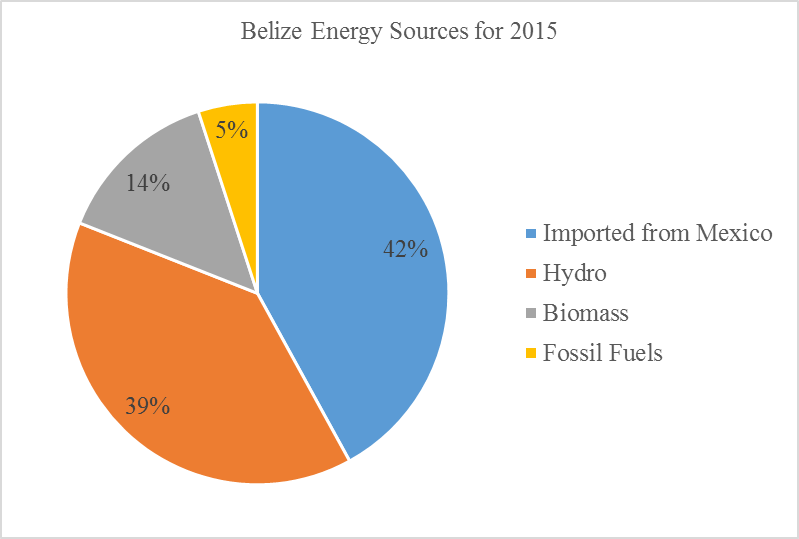
\includegraphics[width = 8cm, height = 6cm]{Energy_Sources_2015.png}
	\caption{PERCENTAGE CONTRIBUTION FROM ENERGY SOURCES IN 2015}
\end{figure} 

\begin{figure}[ht]
	\centering
	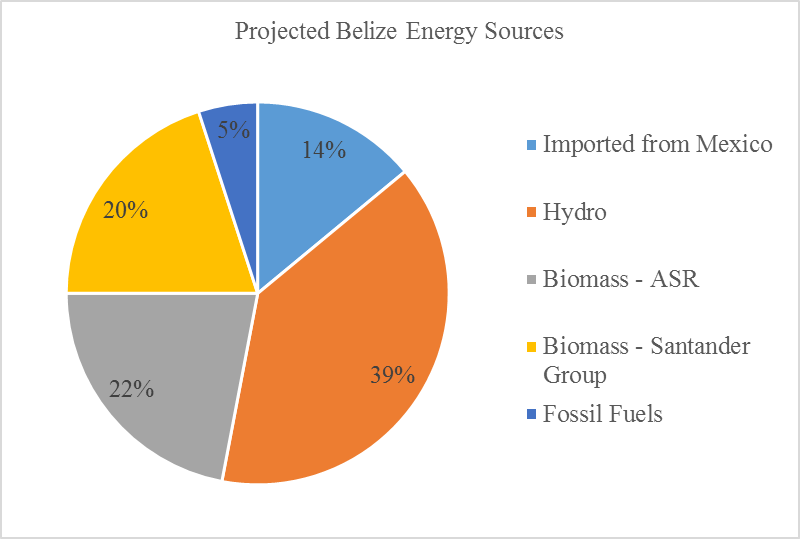
\includegraphics[width = 8cm, height = 6cm]{Energy_Sources_Projected.png}
	\caption{PROJECTED PERCENTAGE CONTRIBUTION FROM ENERGY SOURCES}
\end{figure} 

In 2015, Belize's electricity consumption was 87 thousand MWH, with Mexico supplying approximately 42\%, which is approximately 36.5 thousand MWH. For the past six years, the cost of importing electricity from Mexico has been approximately around \$160 US dollars per MWH \cite{asr_report}. This results in a payment of approximately 5.8 million US dollars to Mexico. A total decrease to only 14\% dependence on Mexico would result in an annual payment of 1.9 million US dollars to Mexico resulting in saving 3.9 million US dollars in foreign payments. The energy sources for the year 2015 are observed in Figure 1 and the projected energy sources considering both investments from ASR and Santander are depicted in Figure 2.  

With adequate policy fostering investment in the expansion of cogeneration technologies, it is evident that there is a positive impact on Belize's economy. However, this impact stems further than the 3.9 million US dollars saved in foreign payments. Growth in income per capita has been observed to be the strongest in outward-looking economies and lowest in inward-looking economies\cite{Crook}. With the agricultural sector being an integral component of Belize's economy, the opportunity to both increase export and simultaneously increase and create domestic sources of renewable energy are advantageous to the economy of Belize. Since there is already the existence of a cogeneration facility and the interest to construct and commission an additional facility, then it is economically advantageous to support the expansion by creating policy that fosters and promotes cogeneration expansion. Furthermore, with the government's interest in supporting green energy, it is beneficial to support cogeneration expansion because of the existence of infrastructure and facilities. 

Three main elements in Sir Arthur Lewis' approach to industrial development in the Caribbean are markets, resource availability, and economy policy formulation \cite{arthur_lewis}. Considering both the agricultural and energy sector in Belize, it is evident that there is a local market for energy consumption, the availability of resource for energy production, and the opportunity to formulate strategic economic policy. Hence, industrial development is viable, which, in turn, would generate economic growth. As a result, it is undoubtedly evident that expansion of cogeneration technologies in Belize would yield notable economic benefits and contribute to the country's economic development. 


\begin{table}[t]
\caption{SANTANDER ANNUAL HARVEST AND ENERGY PROJECTIONS}
\begin{center}
\label{table_ASME}
\begin{tabular}{c l l}
& & \\ % put some space after the caption
\hline
Status & Sugar (T/Year) & Energy(MW)\\
\hline
Projected & 100000 & 16 \\
\hline
\end{tabular}
\end{center}
\end{table}
% Future contribution and why this will be beneficial. References other docs 
\section*{V. TECHNICAL PATHWAYS IN CO-GENERATION}
In order for the investments, by both companies, to maximize economic benefits, practical technological developments of cogeneration in recent years must be taken into consideration. Developments in cogeneration stem further than the direct combustion of bagasse. Investors could consider the introduction of biofuel technology  to convert biomass into biodiesel, bioethanol, or biogas. This section considers the benefits of the introduction of these technologies to support the expansion of cogeneration technologies to yield economic benefit or other technical considerations that could result in economic benefit.
%%%%%%%%%%%%%%%%%%%%%%%%%%%%%%%%%%%%%%%%%%%%%%%%%%%%%%%%%%%%%%%%%%%%%%
Currently, Belcogen produces power using direct combustion of bagasse. In the case of Belcogen, it would be favorable to focus on the achievement of the design output of 27.5 MW, rather than invest in the conversion of biomass to biofuel. As a result, this would mean a focus on the output of the sugar plant, which is not in the context of this paper.   

The previous section on this paper relating to the economic benefits of renewable energy make mention of the details of the Santander Group's investment in sugar cane growth in Belize. Also discussed was Santander's intent to further invest and bring online another cogeneration plant in the country which could effectively provide the national grid with about 20\% of its needs. While this technical pathway of using the sugarcane bagasse for electric energy production through cogeneration would indeed achieve the marked increases in renewable energy production previously mentioned, there exists other routes through which this can be accomplished. Biochemical processing of the sugarcane bagasse can result in ethanol production. Comparative studies have shown that a mature technology which efficiently produces ethanol from ligno-cellulosic materials, of which sugarcane bagasse is a subset, would be considerably more profitable and could even mitigate the production of more green house gasses than the typical cogeneration process \cite{biomass_comp}.

While studies have shown the potential for increased profitability from biofuels in comparison to cogeneration, developing economies might not be able to expend the required capital to implement such new technologies. Recent studies have argued that the only economically feasible option at present in Brazil is to use the sugarcane bagasse in the production of electricity generation from biomass combustion\cite{brazil_no}. It could be argued that given the scale of Belize's economy in comparison to Brazil's, the same argument would hold in Belize. Further investigation of this would be required to confirm whether or not the production of bio-oil from sugarcane bagasse would be a viable option for the country. 

%%%%%%%%%%%%%%%%%%%%%%%%%%%%%%%%%%%%%%%%%%%%%%%%%%%%%%%%%%%%%%%%%%%%%%
\section*{VI. CONCLUSION}

Belize's agricultural history has shown that sugarcane is a vital crop to Belize's economy. With Belize's interest in the implementation of renewable energy, there is the unique opportunity to amalgamate both the agricultural and energy sectors in Belize to yield sustainable and realistic economic growth. With strategic policies in place, expansion of the current cogeneration technologies in Belize would drastically reduce the country's dependence on foreign energy. The investment in cogeneration technologies could lead to a direct savings of 3.9 million US dollars per year. Furthermore, investment in cogeneration also yields other benefits such as industrial development which also promote economic growth. The paper has shown that with the necessary regulations in place, Belize can take advantage of its already existing agricultural facilities to stimulate economic growth through the production of renewable energy. The positive conditions such as flexibility in policy development, interest in investment, and pre-existing facilities serve as indicators that the expansion of cogeneration in Belize is the most advantageous pathway toward stimulating practical and sustainable economic growth.  Moreover, this paper serves as a foundation to further promote research in the area of renewable energy and economic development in Belize considering the lack of research surrounding the regulatory, economic and technical components of Belize's renewable energy sector.



%%%%%%%%%%%%%%%%%%%%%%%%%%%%%%%%%%%%%%%%%%%%%%%%%%%%%%%%%%%%%%%%%%%%%%




% Here's where you specify the bibliography style file.
% The full file name for the bibliography style file 
% used for an ASME paper is asmems4.bst.
\bibliographystyle{asmems4}


%%%%%%%%%%%%%%%%%%%%%%%%%%%%%%%%%%%%%%%%%%%%%%%%%%%%%%%%%%%%%%%%%%%%%%


%%%%%%%%%%%%%%%%%%%%%%%%%%%%%%%%%%%%%%%%%%%%%%%%%%%%%%%%%%%%%%%%%%%%%%
% The bibliography is stored in an external database file
% in the BibTeX format (file_name.bib).  The bibliography is
% created by the following command and it will appear in this
% position in the document. You may, of course, create your
% own bibliography by using thebibliography environment as in
%
% \begin{thebibliography}{12}
% ...
% \bibitem{itemreference} D. E. Knudsen.
% {\em 1966 World Bnus Almanac.}
% {Permafrost Press, Novosibirsk.}
% ...
% \end{thebibliography}

% Here's where you specify the bibliography database file.
% The full file name of the bibliography database for this
% article is asme2e.bib. The name for your database is up
% to you.
\bibliography{asme2e}



\end{document}
